\section{Project summary}

In this project we will attempt to answer the research questions shown in figure \ref{fig:Research_Questions}.
\begin{figure}[H]
    \centering
    \fbox{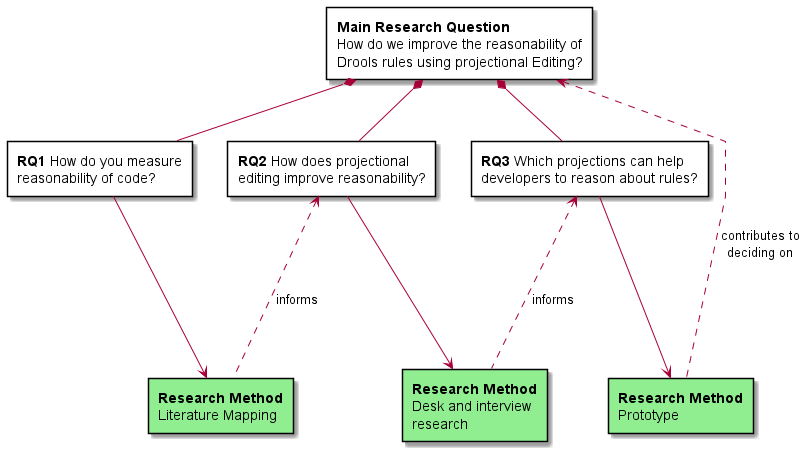
\includegraphics[width=0.95\textwidth]{images/ResearchQuestion.png}}
    \caption{Research Questions and Methods}
    \label{fig:Research_Questions}
\end{figure}


Drools\cite{browne2009jboss} is an open-source production rule system for complex event processing, using an implementation of the Rete algorithm\cite{forgy1989rete}.
It has its own Domain Specific Language (DSL), in which rules are described.
These are stored in Drools (.drl) files. 
Reasoning about a small number of rule is hard, at the host organization there are many file with dozens of rules in them.
This project will attempt to improve how one can reason about rule in an editor.

Editing in language workbenches comes in two forms, either free-form text editing or, less frequently, projectional editing\cite{erdweg2013state}.
Projectional editing is a method of bypassing the parser and programming directly into projections of the Abstract Syntax Tree.
We will recreate this DSL using a language workbench capable of creating projectional editors.  
On top of this newly modelled DSL, we will create new and different projections of the code for the purpose of increasing the reasonability of the code. 

In this project we will use the open-source language workbench Meta Programming System (MPS) from JetBrains\cite{MPS_ProductPage}.
MPS is built around the projectional editing paradigm.
There is no existing implementation of the Drools language in MPS.
Although Drools is nearly 20 years old and has wide use, it does not have strong IDE support.
One artefact of this masters project will be a prototype projectional editor, that will give much stronger editor support in IntelliJ, currently the most used IDE\cite{Java_usage_report}.
